\documentclass[14pt,a4paper,russian]{scrartcl}
% \documentclass[14pt,a4paper,oneside,russian,fontsize=14pt]{scrartcl}
\usepackage{mystyle}
\graphicspath{{images/}}

\begin{document}

\renewcommand{\onlyinsubfile}[1]{}
\renewcommand{\notinsubfile}[1]{#1}

% 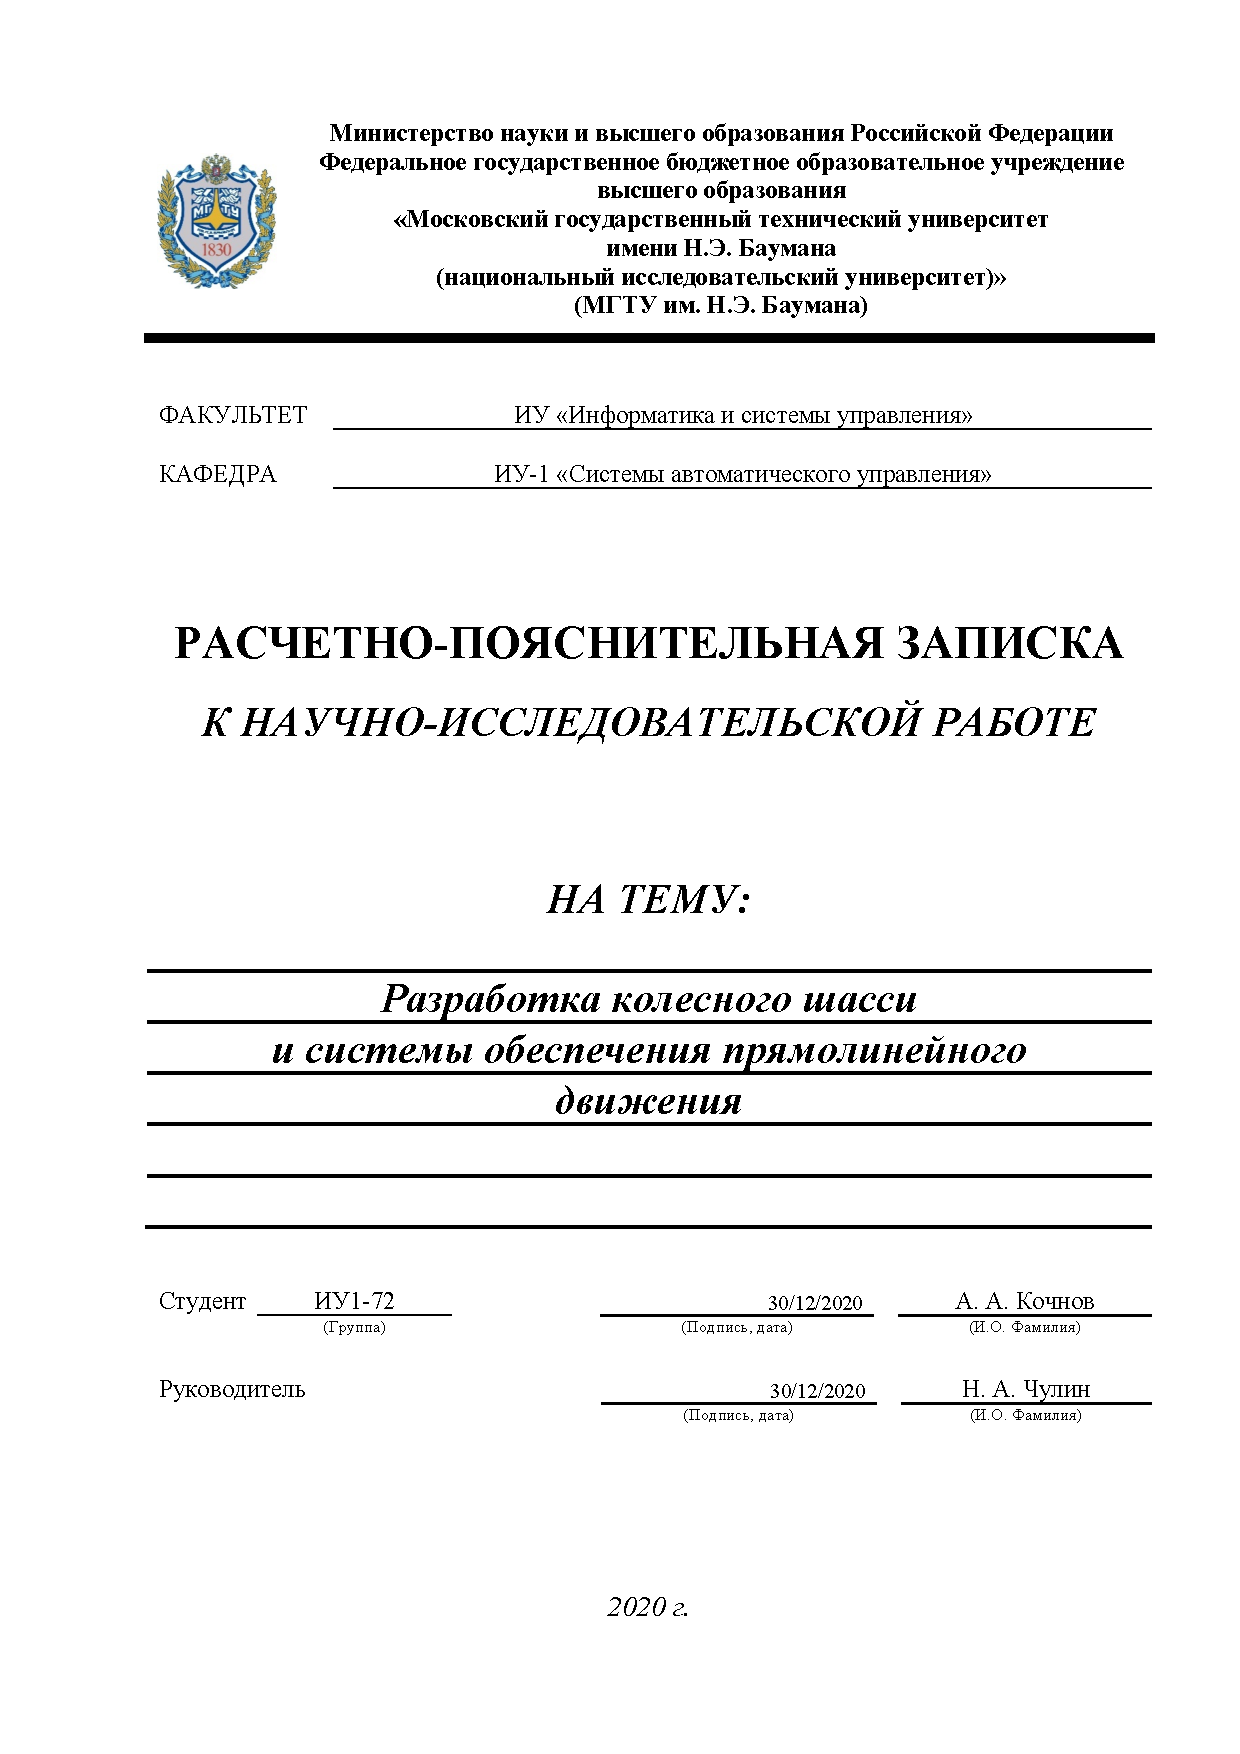
\includepdf[page={1}]{parts/titul}

\tableofcontents
\newpage

\section*{Вступление}
\addcontentsline{toc}{section}{Вступление}
Системы автоматического управления используются повсеместно. Основная 
их задача - поддерживать состояние системы в соответствии 
с некоторыми требованиями - движение по заданной траектории, поддержание температуры и т.д.

Одна из причин, почему контролируемая система начинает со временем
не соответствовать заданным условиям - это различные внешние воздействия. Например,
окружающая среда может похолодать, из-за чего автоматическая печь начнет остывать
быстрее. Или беспилотник начнет сносить в сторону боковой ветер. Кроме того, 
стабильности состояния может помешать несовершенство механизма, который управляется.
Например, люфт в механических передачах, неодинаковые параметры двигателей и т.д.

Для решения проблемы в систему управления вводится обратная связь и некоторый 
регулятор, чтобы компенсировать влияние помех. Поэтому ставятся задачи как чисто 
аналитического плана - синтез регулятора, так и технического - разработка
удачного ПО для непосредственного управления электромеханическими частями обьекта,
измерение необходимых параметров среды и состояния системы, предварительная обработка
и очистка сигнала, чтобы сделать его пригодным для анализа.

В данной НИР мы начинаем подготовительную работу для анализа работы и влияния
различных методов и приемов компенсации помех в работе подвижных объектов. 
Так как максимально продуктивным будет изучение на практике, необходимо разработать
подвижную мобильную платформу, способную перемещаться в пространстве в соответствии
с заданными командами, а также собирать и обрабатывать информацию о своем состоянии.
Выбран наземный вариант с перемещением в 2D-пространстве как наиболее простой вариант,
упрощающий реализацию но не основные принципы и идеи.

\newpage

\section*{Основная часть}
\addcontentsline{toc}{section}{Основная часть}
\subsection{Постановка задачи}
Как уже было указано, 
\newpage

\subsection{Практическая часть}
Основная задача на НИР этого семестра - создание платформы для отработки
приемов и методов управления. Процесс можно разделить на
несколько частей - сборка механической части, разработка ПО для микроконтроллера и 
разработка подобия управляющего терминала.
\subsubsection{Создание шасси}
В основе подвижного мобильного шасси лежит готовый комплект. Пример
представлен на рис. \ref{fig:shassis_dissassembled}. Он включает в себя пластиковую основу,
стойки-крепления, электрические двигатели постоянного тока с пластиковыми редукторами,
колёса с прорезиненным протектором (который, тем не менее, довольно хорошо скользит)
и дисками для тахометров.
\begin{figure}[h]
    \center{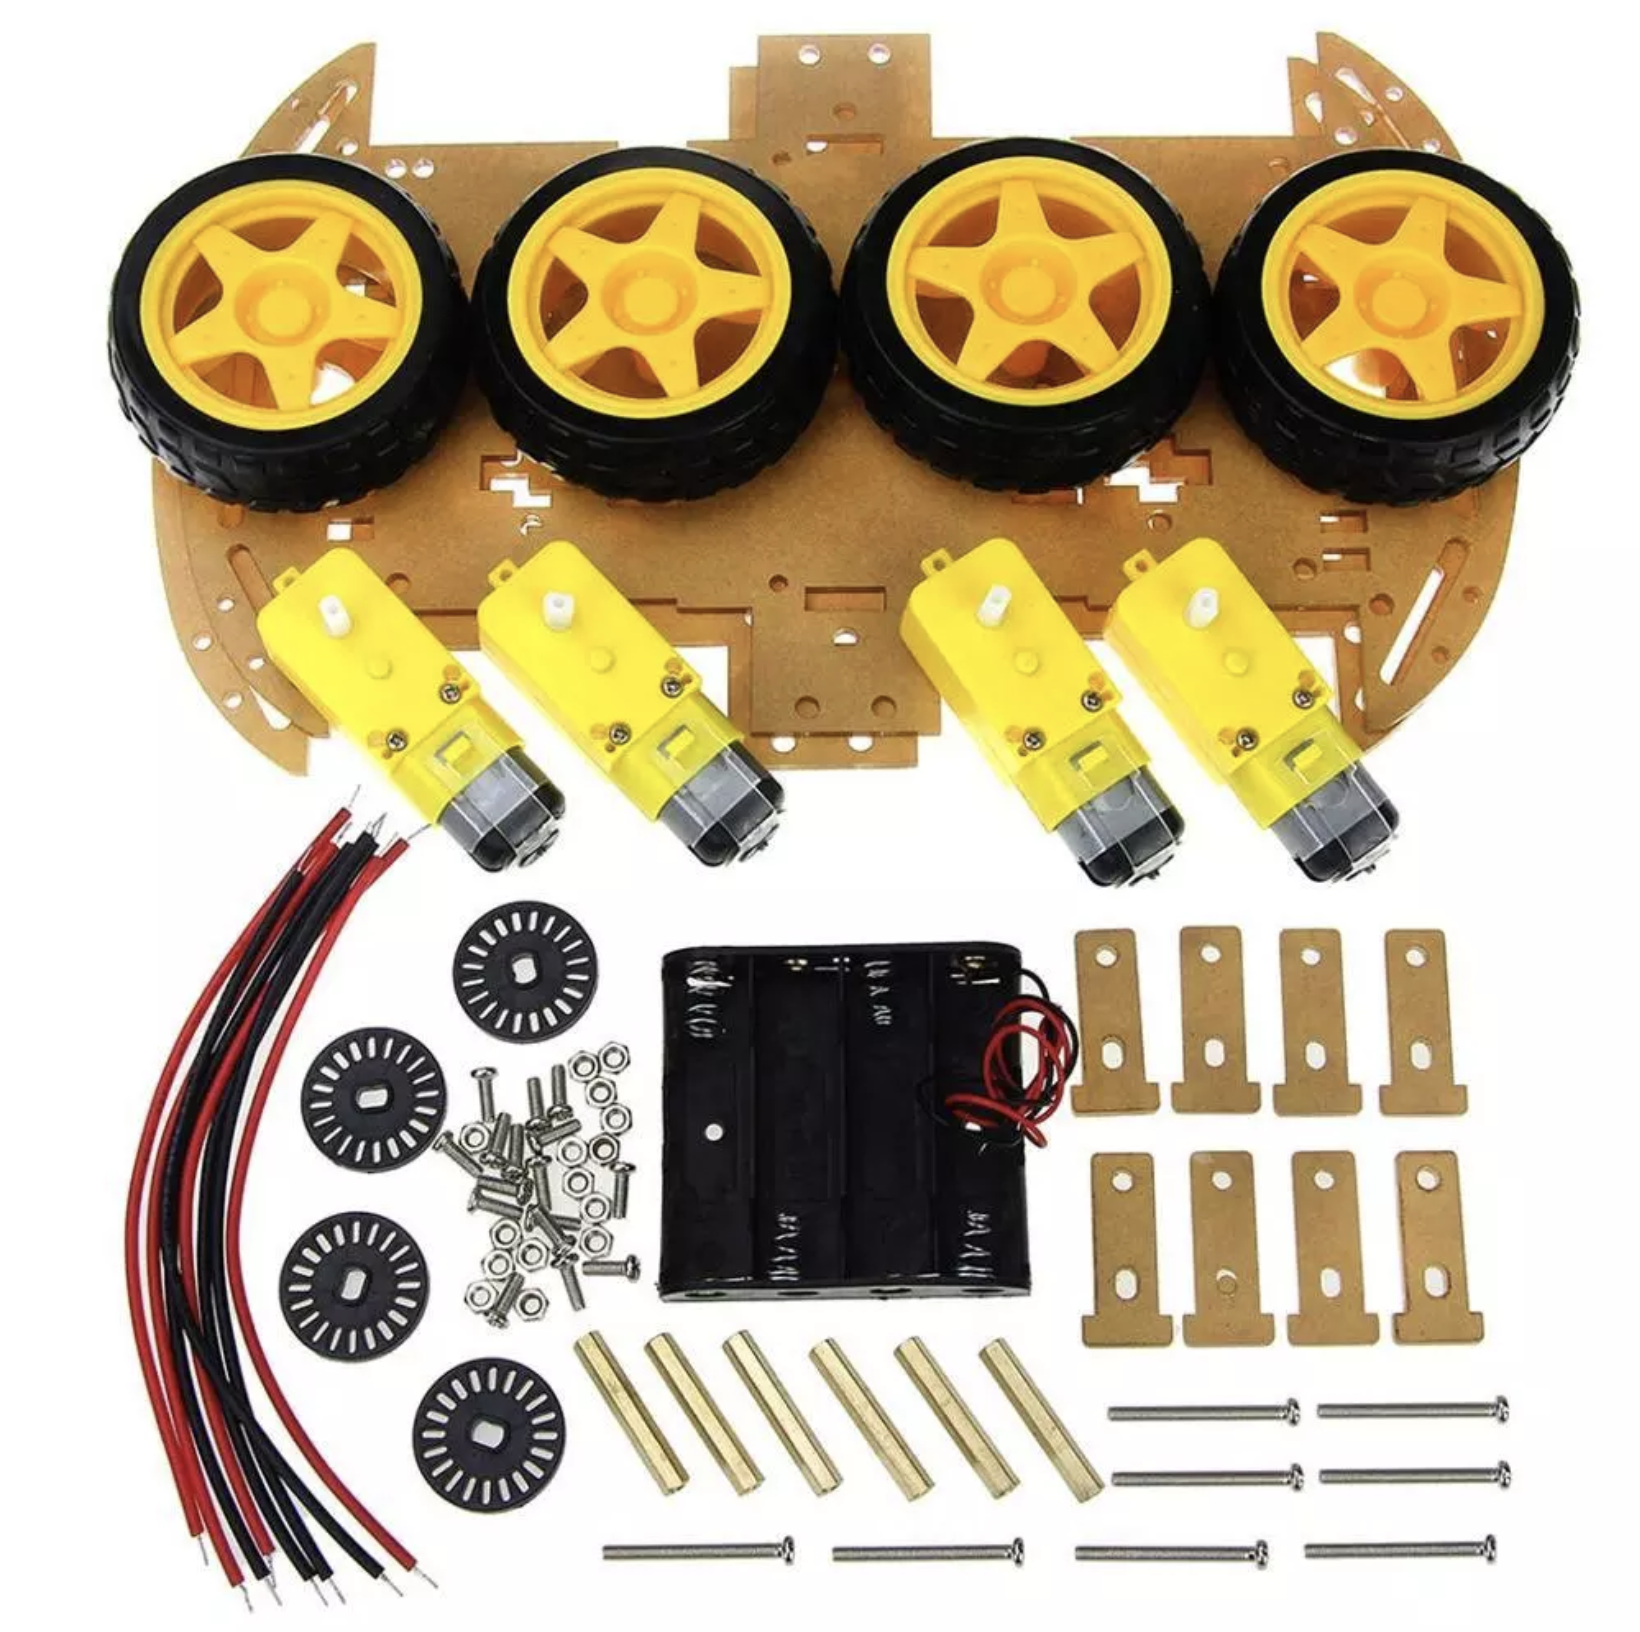
\includegraphics[width=0.8\linewidth]{shassis_dissassembled.png}}
    \caption{Основа шасси в разобранном виде}
    \label{fig:shassis_dissassembled}
\end{figure}

Как видно из фотографии, оригинальный комплект подразумевает наличие четырёх
ведущих колёс. Однако, как выяснилось в тестах, колеса начинают прокальзывать,
что вкупе с довольно неоднородными реальными характеристиками двигателей
превращало процесс движения шасси в довольно стохастичекий процесс. Поэтому
решено было оставить лишь два задних колеса, а для сохранения баланса
поставить вперёд ведомое колесо-подставку, которое дополнительно
легко вращается вокруг вертикальной оси, не препятствуя движению объекта. Заметим,
что массивные батареи также находятся сзади, что обеспечит колёсам хорошее
сцепление с поверхностью.

Комплект хороший, но этого недостаточно для поставленных задач. Далее шасси
необходимо дополнить электронными компонентами. 

Во-первых, необходим микроконтроллер. Рассматривались несколько вариантов:
\begin{itemize}
    \item Arduino (контроллеры семейства AVR серии ATmega, кроме Due)
    \begin{itemize}
        \item Uno (ATmega328 16 МГц, Flash 32Кб, RAM 2Кб, 14 IO pins)
        \item Mega 2560 (ATmega2560 16 МГц, Flash 256 Кб, RAM 8 Кб, 54 IO pins)
        \item Due (ARM AT91SAM3X8E 84 МГц, Flash 512 КБ, RAM 96 КБ, 54 IO pins)
        \item Pro mini (ATmega328 16 МГц, Flash 32 Кб, RAM 2 Кб, 14 IO pins)
    \end{itemize}
    \item STM32 (контроллеры семейства ARM)
    \begin{itemize}
        \item STM32F103C8T6 "Blue Pill" (Cortex M3 72Мгц, Flash 64Кб, RAM 32Кбб 37 IP pins)
    \end{itemize}
\end{itemize}
Наиболее популярный вариант - Arduino Uno. Обладает мощностями, достаточными
для решения задачи на начальном этапе, однако имеет достаточно большие размеры и
некоторые излишества, которые хороши для обучения работы с микроконтроллерами,
но не нужны в готовом устройстве. STM32 куда мощнее и быстрее, компактна
и вообще хороша во всём, кроме фреймфорков. Существуют удобные готовые подобия
RTOS (ОС реального времени), однако они довольно большие и занимают почти всю
доступную память данного контроллера начального уровня. Библиотеки более низкого
уровня сложныи требуют слишком много времени на освоение, что не предполагается
в данной задаче.

Итого, была выбрана плата Arduino Pro Mini, представленная на рис.\ref{fig:pro_mini}
\begin{figure}[h]
    \center{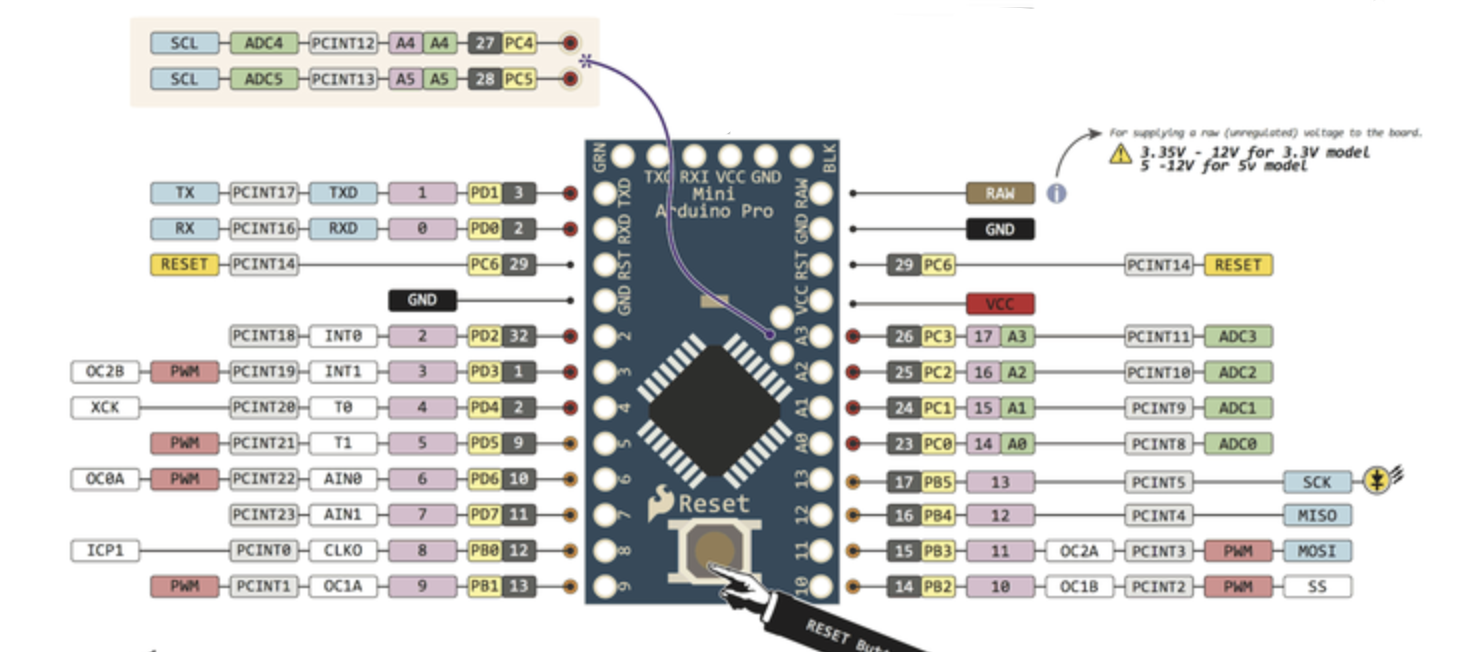
\includegraphics[width=1\linewidth]{pro_mini.png}}
    \caption{Arduino Pro mini со схемой распиновки}
    \label{fig:pro_mini}
\end{figure}

Основа любого мобильного шасси - это двигатели. В данной сборке их два - на каждое
колесо. Чтобы управлять направлением движения, необходимо менять полярность подключения
к источнику питания. Чтобы управлять скоростью (и усилием) вращения, используется
ШИМ-сигнал. Так как для двигателей необходимо высокое напряжение (7..8 В), большее,
чем требует контроллер (3.3 В), а также большой ток, двигатели подключаются
к так называемому драйверу электродвигателей. Он основан на Н-мосте, который позволяет
менять полярность подключения, а также транзисторных ключах, которые на основе ШИМ-сигнала
малого напряжения модулируют рабочее напряжение. В данной сборке использован драйвер
на базе микросхемы L298N, имеющий ровно два независимых канала. 
Представлен на рис.\ref{fig:motor_driver}.
\begin{figure}[h]
    \center{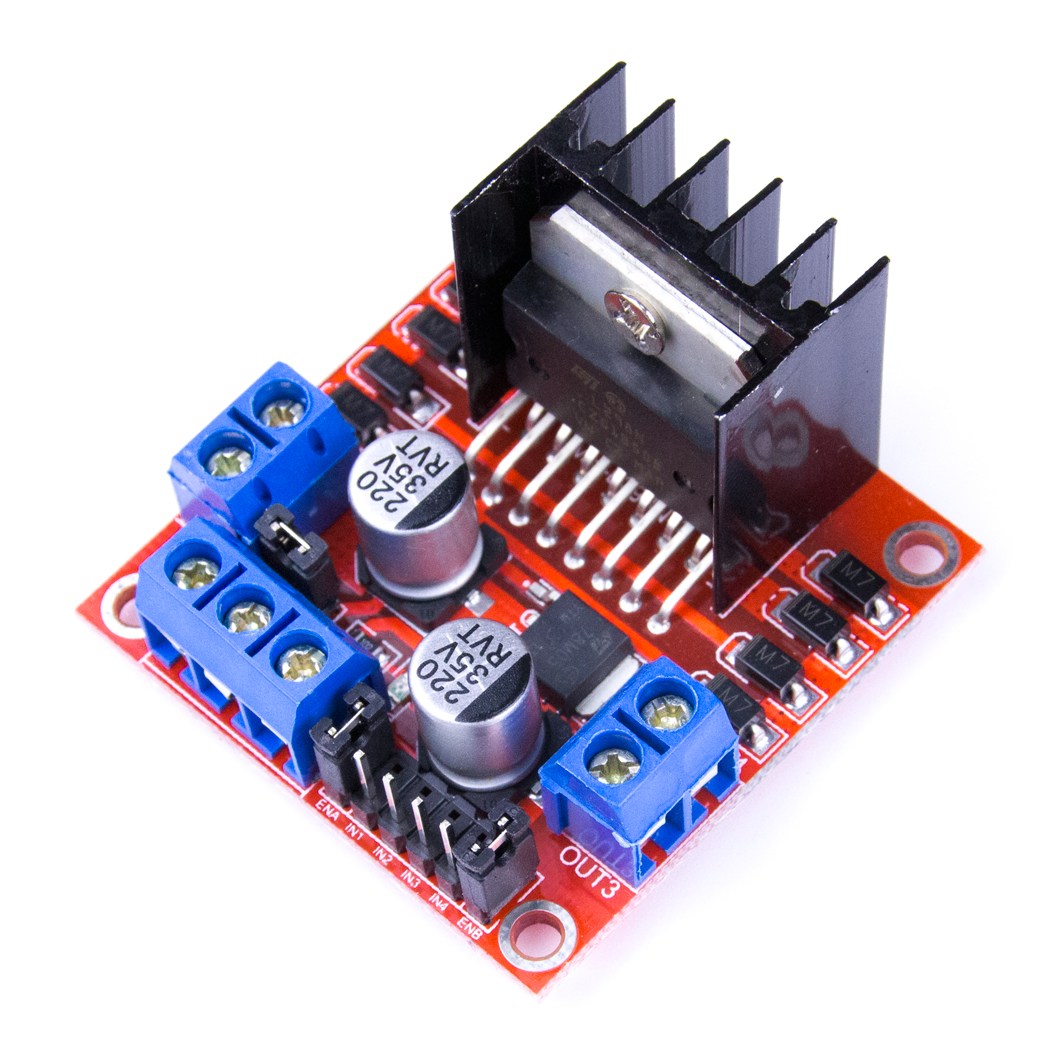
\includegraphics[width=0.6\linewidth]{motor_driver.png}}
    \caption{Драйвер электродвигателей L298N}
    \label{fig:motor_driver}
\end{figure}

Для определения состояния шасси для обеспечения обратной связи
необходимы датчики. Так как мы рассматриваем процесс движения, 
необходимо получать данные о пройденном пути, текущей скорости обьекта (как 
линейной, так и угловой), ускорения. 

Для контроля работы двигательной
подсистемы будем использовать оптические тахометры. Принцип действия использованных
оптических тахометров заключается в реакции на каждое прохождение препятствия
между светодиодом и оптическим приемником. Зная момент прохождения и количество
щелей в диске, можно довольно точно вычислять суммарный угол поворота колеса.
Проводя численное дифференциирование, можно получать угловые скорости (и даже
угловые ускорения) вращения каждого из колес. В итоге можно узнавать 
общую угловую (и линейную) теоретические скорость шасси, откуда компенсировать различия в параметрах (а
следовательно, и в реальной скорости вращения) двигателей, обеспечивая
прямолинейное движение. Приведён на рис.\ref(fig:encoder).
\begin{figure}[h]
    \center{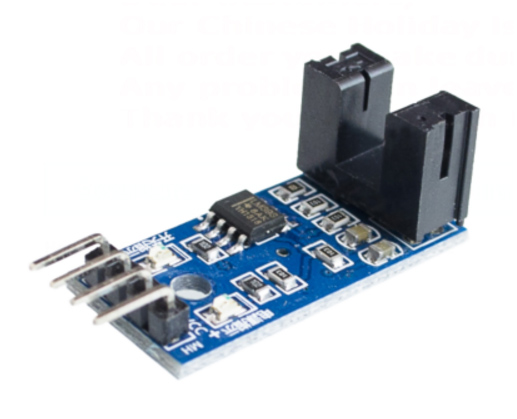
\includegraphics[width=0.6\linewidth]{encoder.jpg}}
    \caption{Оптический тахометр (энкодер)}
    \label{fig:encoder}
\end{figure}

Теоретические скорости - хорошая вещь. Но она получается в предположении
что колеса идеально сцепляются с повехностью без проскальзывания, 
а шасси не подвергаются внешним воздействиям и не упирается в препятствия.
Для получения данных о реальном состоянии движения используем связку 
гироскоп-акселерометр. Простейшие варианты поставляются в виде объединенной
платы, которая отличается не только весьма удовлетворительной точностью, но
и сверхнизкой стоимостью. Пример представлен на рис.\ref{fig:gyro_accel}.
\begin{figure}[h]
    \center{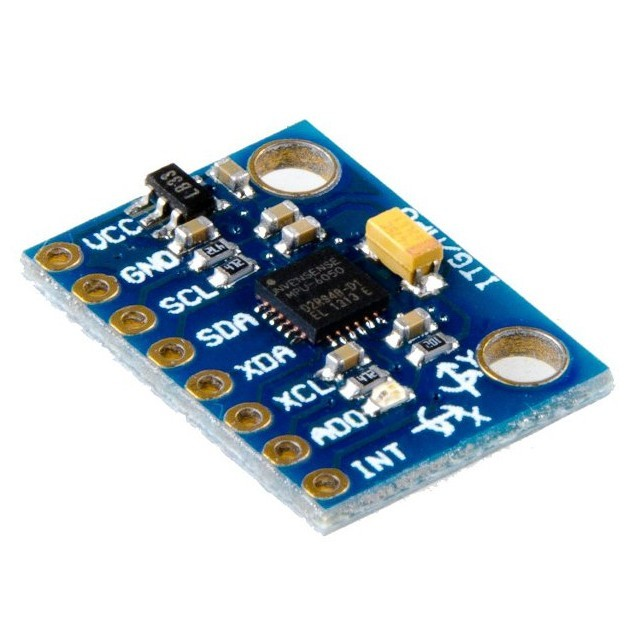
\includegraphics[width=0.6\linewidth]{gyro.jpg}}
    \caption{Гироскоп-акселерометр GY-521 (MPU-6050)}
    \label{fig:gyro_accel}
\end{figure}

Дополнительно можно использовать электронный датчик магнитного поля.
Вкупе модулем выше можно реализовать электронный компас, с помощью которого
измерять абсолютный угол поворота робота. Однако он подвержен помехам от 
двигателей, а также довольно сложен в реализации, поэтому в данной версии
не использовался. Выглядит очень схоже с платой гироскопа. Кроме того,
в роботы такого типа также ставятся ультразвуковые/инфракрасные датчики расстояния
или даже лидары. Однако в данной работе ставится задача лишь контроля
траектории шасси, поэтому эти устройства также не используются.

По заданию необходимо задавать роботу направление движения извне. Так как
шасси подвижное, необходима беспрроводная связь. Рассматривалось
и тестировалось несколько вариантов. Сначала предполагалось использование 
передатчика nRF24l01, позволяющего держать связь до 50м на открытом пространстве.
В этом случае команды не должны теряться в пределах помещения и доходить
быстро и надежно. Однако цепочка шасси <-радио-> приемник <-USB-> терминал
оказалась довольно сложной. Потому исходя из предположения небольших
размеров помещения для тестирования шасси использован простой bluetooth-передатчик,
держащий связь непосредственно с терминалом.

Терминал изначально предполагался физический. Однако имеющиеся джойстики
не предполагали высокого качества и точности выдаваемого сигнала, поэтому
эта идея была пропущена.

Дополнительно для схемы использовался понижающий преобразователь
напряжения для получения напряжения 5В для микроконтроллера и датчиков, 
Li-Ion батареи типоразмера 18650 и автономного вольтметра для 
визуального контроля состояния батарей.

Итоговый вариант сборки представлен на рис.

\section*{Заключение}
\addcontentsline{toc}{section}{Заключение}

\newpage


\newpage
\end{document}